\documentclass{beamer}
\DeclareFontShape{OT1}{cmss}{b}{n}{<->ssub * cmss/bx/n}{} 
\usetheme{Szeged}
\usecolortheme{beaver}
\usepackage{amsmath}
\usepackage{amsfonts}
\usepackage{mathbbol}
\usepackage{xcolor} % before tikz or tkz-euclide if necessary
\usepackage{tkz-euclide} % no need to load TikZ
\usepackage{multirow}
\usepackage{lmodern}
\usepackage{bm}
\usepackage{subcaption}
%\usepackage{subfigure}

\usepackage[
backend=biber,
style=authoryear-icomp,
sortlocale=de_DE,
natbib=true,
url=false, 
doi=true,
eprint=false
]{biblatex}
\addbibresource{../Bibliography/main_ML.bib}



\titlegraphic{
\includegraphics[width=2cm]{../Figures/UAMS_RGB.png}
}


\title{Neuroinformatics Journal Club\\ Edge-centric brain FC }
\author{Horacio G\'omez-Acevedo\\ Department of Biomedical Informatics\\
	University of Arkansas for Medical Sciences}

\begin{document}
	\begin{frame}[plain]
		\maketitle
	\end{frame}
	
	\begin{frame}{Today's paper}
		\begin{figure}[h]
			\centering
			%	\begin{subfigure}{0.4\textwidth}
				%		\centering
				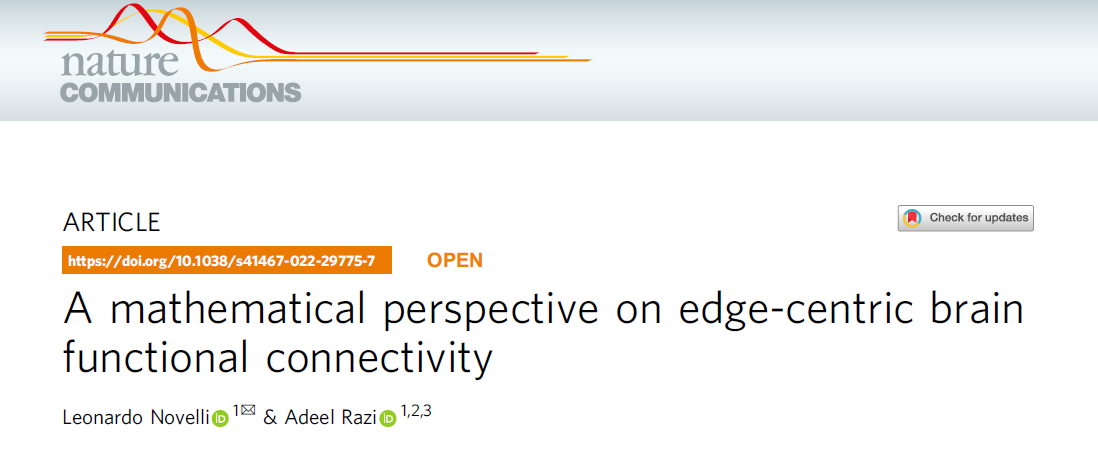
\includegraphics[scale=0.45]{../Figures/novelli_paper.png}
				%	\end{subfigure}
		\end{figure}
	\end{frame}
	
	
	%	\begin{frame}{Hidden Markov Models}
		%		The implementation of Hidden Markov models dates back in the late 60's by Leonard Baum and collaborators. It is still an active area of research. 	
		%		
		%		What is a Markov chain?
		%		\begin{figure}[h]
			%			\centering
			%			%	\begin{subfigure}{0.4\textwidth}
				%				%		\centering
				%				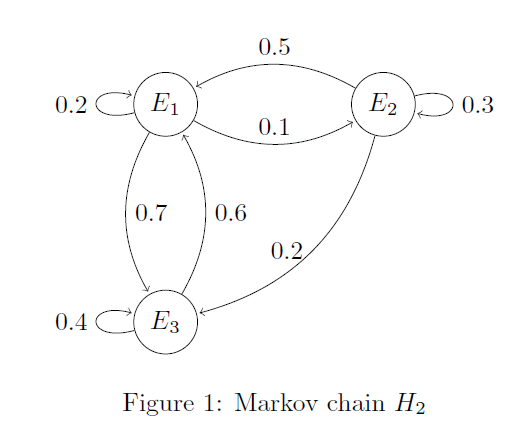
\includegraphics[scale=0.6]{../Figures/fig_markov_chain.png}
				%				%	\end{subfigure}
			%		\end{figure}
		%		
		%		
		%	\end{frame}
	%	
	%	\begin{frame}{Hidden Markov Chains}
		%		The fair casino problem 
		%		\begin{itemize}
			%			\item You don't know if the dealer has a fair or unfair coin (Hidden states)
			%			\item You only observe the output (Emissions)
			%		\end{itemize}
		%		\begin{figure}[h]
			%			\centering
			%			%	\begin{subfigure}{0.4\textwidth}
				%				%		\centering
				%				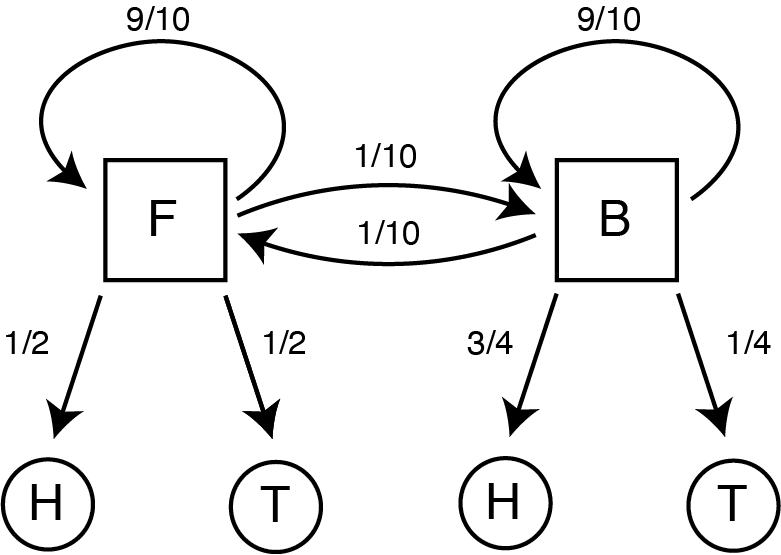
\includegraphics[scale=0.6]{../Figures/hmm_fair_casino.png}
				%				%	\end{subfigure}
			%		\end{figure}
		%	\end{frame}
	%	
	\begin{frame}{Inconsistencies from the beginning}
		There are some major flaws with the paper. For once, the notation is confusing.
		\begin{itemize}
			\item So $c_{ij}= z_i(t) z_j (t)$. This is a vector.
			\item $C_{ij}(t)$ is a matrix?
			\item $\textrm{C}_{ij}$ is a matrix in formula 12. 
		\end{itemize}
		\begin{figure}[h]
		\centering
		%	\begin{subfigure}{0.4\textwidth}
			%		\centering
			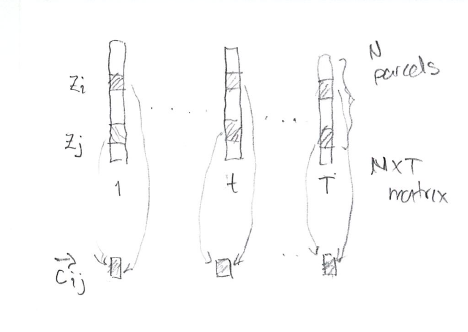
\includegraphics[scale=0.4]{../Figures/fig_novelli_description1.png}
			%	\end{subfigure}
	\end{figure}
	\end{frame}

	\begin{frame}{A vector then...}
		\begin{figure}[h]
	\centering
	%	\begin{subfigure}{0.4\textwidth}
		%		\centering
		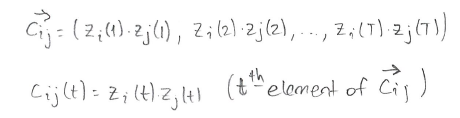
\includegraphics[scale=0.4]{../Figures/fig_novelli_description2.png}
		%	\end{subfigure}
\end{figure}
		
	\end{frame}

\begin{frame}{A collection of vectors}
		\begin{figure}[h]
		\centering
		%	\begin{subfigure}{0.4\textwidth}
			%		\centering
			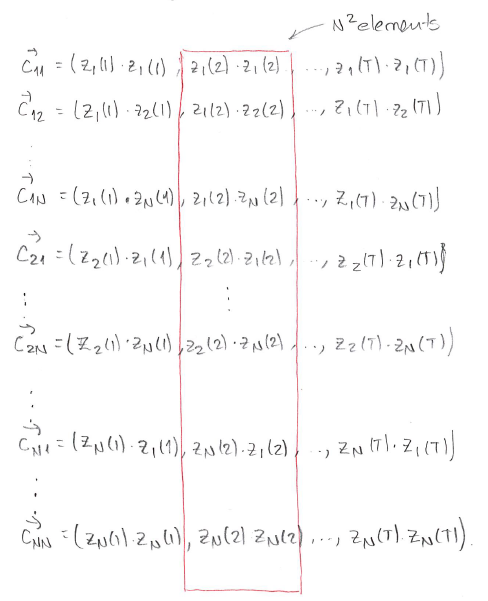
\includegraphics[scale=0.3]{../Figures/fig_novelli_description3.png}
			%	\end{subfigure}
	\end{figure}
	
\end{frame}

\begin{frame}{Edge Time Series?	}
	\begin{figure}[h]
		\centering
		%	\begin{subfigure}{0.4\textwidth}
			%		\centering
			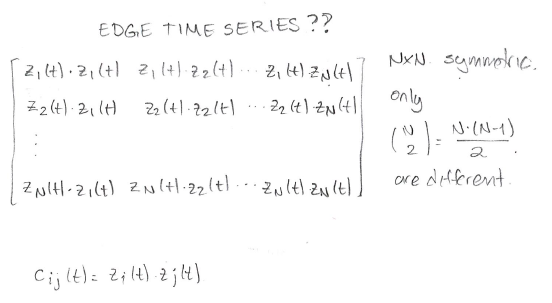
\includegraphics[scale=0.6]{../Figures/fig_novelli_description4.png}
			%	\end{subfigure}
	\end{figure}
\end{frame}

\begin{frame}{Definition of eFC?}
	\begin{figure}[h]
	\centering
	%	\begin{subfigure}{0.4\textwidth}
		%		\centering
		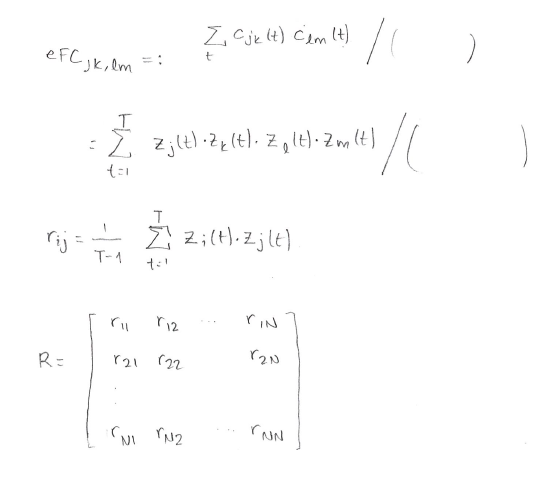
\includegraphics[scale=0.4]{../Figures/fig_novelli_description5.png}
		%	\end{subfigure}
\end{figure}
\end{frame}

\begin{frame}{Changing notation}
\begin{figure}[h]
	\centering
	%	\begin{subfigure}{0.4\textwidth}
		%		\centering
		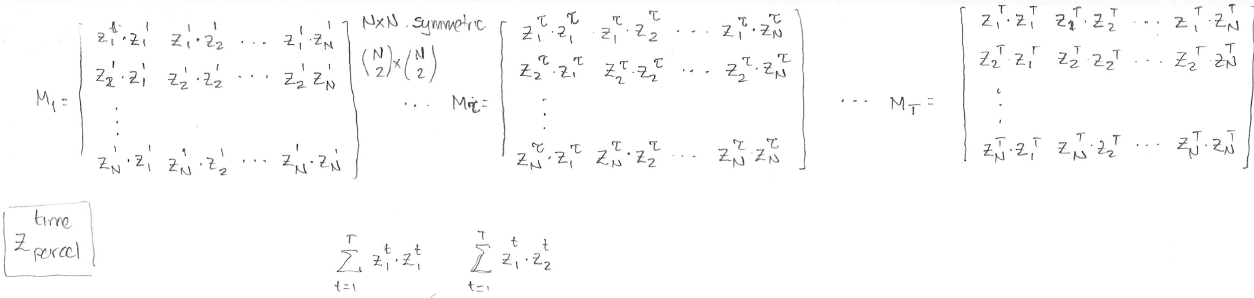
\includegraphics[scale=0.4]{../Figures/fig_novelli_description6.png}
		%	\end{subfigure}
\end{figure}	
\end{frame}

\begin{frame}{Fourth order statistics eFC}
\begin{figure}[h]
	\centering
	%	\begin{subfigure}{0.4\textwidth}
		%		\centering
		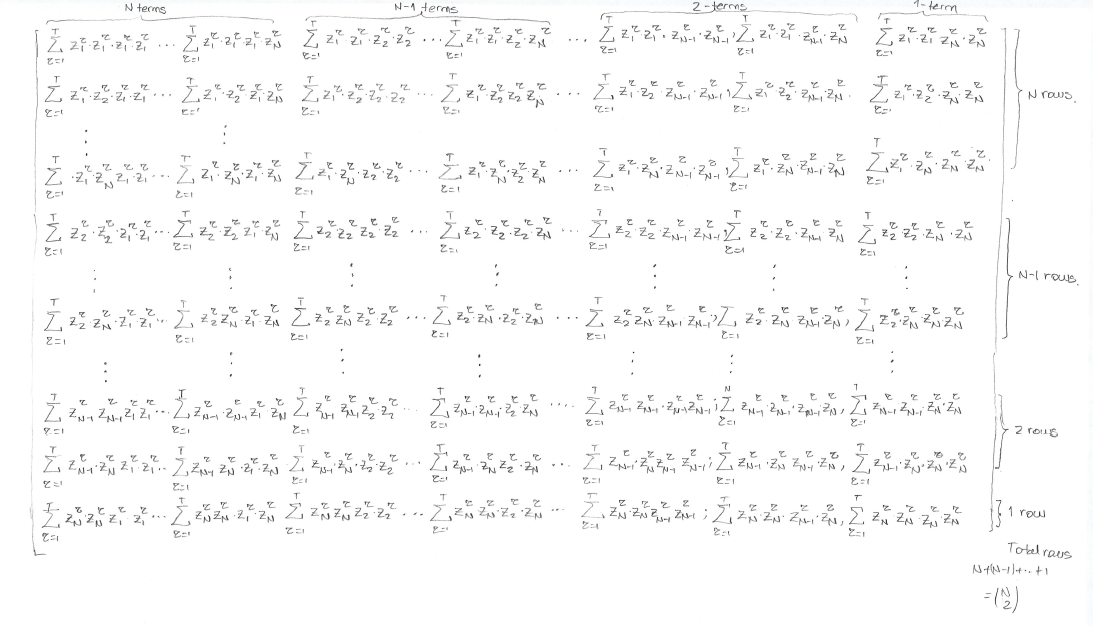
\includegraphics[scale=0.3]{../Figures/fig_novelli_description7.png}
		%	\end{subfigure}
\end{figure}	
\end{frame}

\begin{frame}{Derivation of edge FC}
	\begin{equation}
		E[C_{jk}(t) C_{jl}(t)]= E[Z_i(t)Z_k(t)Z_j(t)Z_l(t)]+ \textrm{ sum of products of two}
	\end{equation}.

The assumption of  $\kappa (E[Z_i(t)Z_k(t)Z_j(t)Z_l(t)])=0$ is unrealistic. Confussion at its best... $E(Z_i)=0$, Ok, but if they are assuming independence the whole thing is zero!
 
\end{frame}

\begin{frame}{Ergodicity }
	This condition is very strong, and it refers to this scary looking condition
	\begin{equation}
		\lim_{t\to \infty} E[C_{jk}(t) C_{jl}(t)] \textrm{ exists!}
	\end{equation}
They are clever enough to put it under the carpet by saying
"the ergodic assumption guarantees that sample estimates converge to the ensemble expectation as the number of time frame increases". 

Equation 10 holds  in the limit case... otherwise it is an estimate!

\end{frame}
		
\begin{frame}{Distance? right!}
	The equation 12 needs to be divided by $(T-1)^2$, furthermore there are tons of repetitions in the equation (remember we eliminated the lower half of the matrices)
\end{frame}

\begin{frame}{This is what I need to do}
\begin{figure}[h]
	\centering
	%	\begin{subfigure}{0.4\textwidth}
		%		\centering
		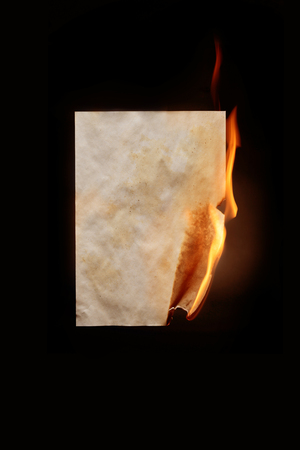
\includegraphics[scale=1.4]{../Figures/main_idea.jpeg}
		%	\end{subfigure}
\end{figure}	
\end{frame}	
	
\begin{frame}{Colophon}
	\begin{figure}[h]
		\centering
		%	\begin{subfigure}{0.4\textwidth}
			%		\centering
			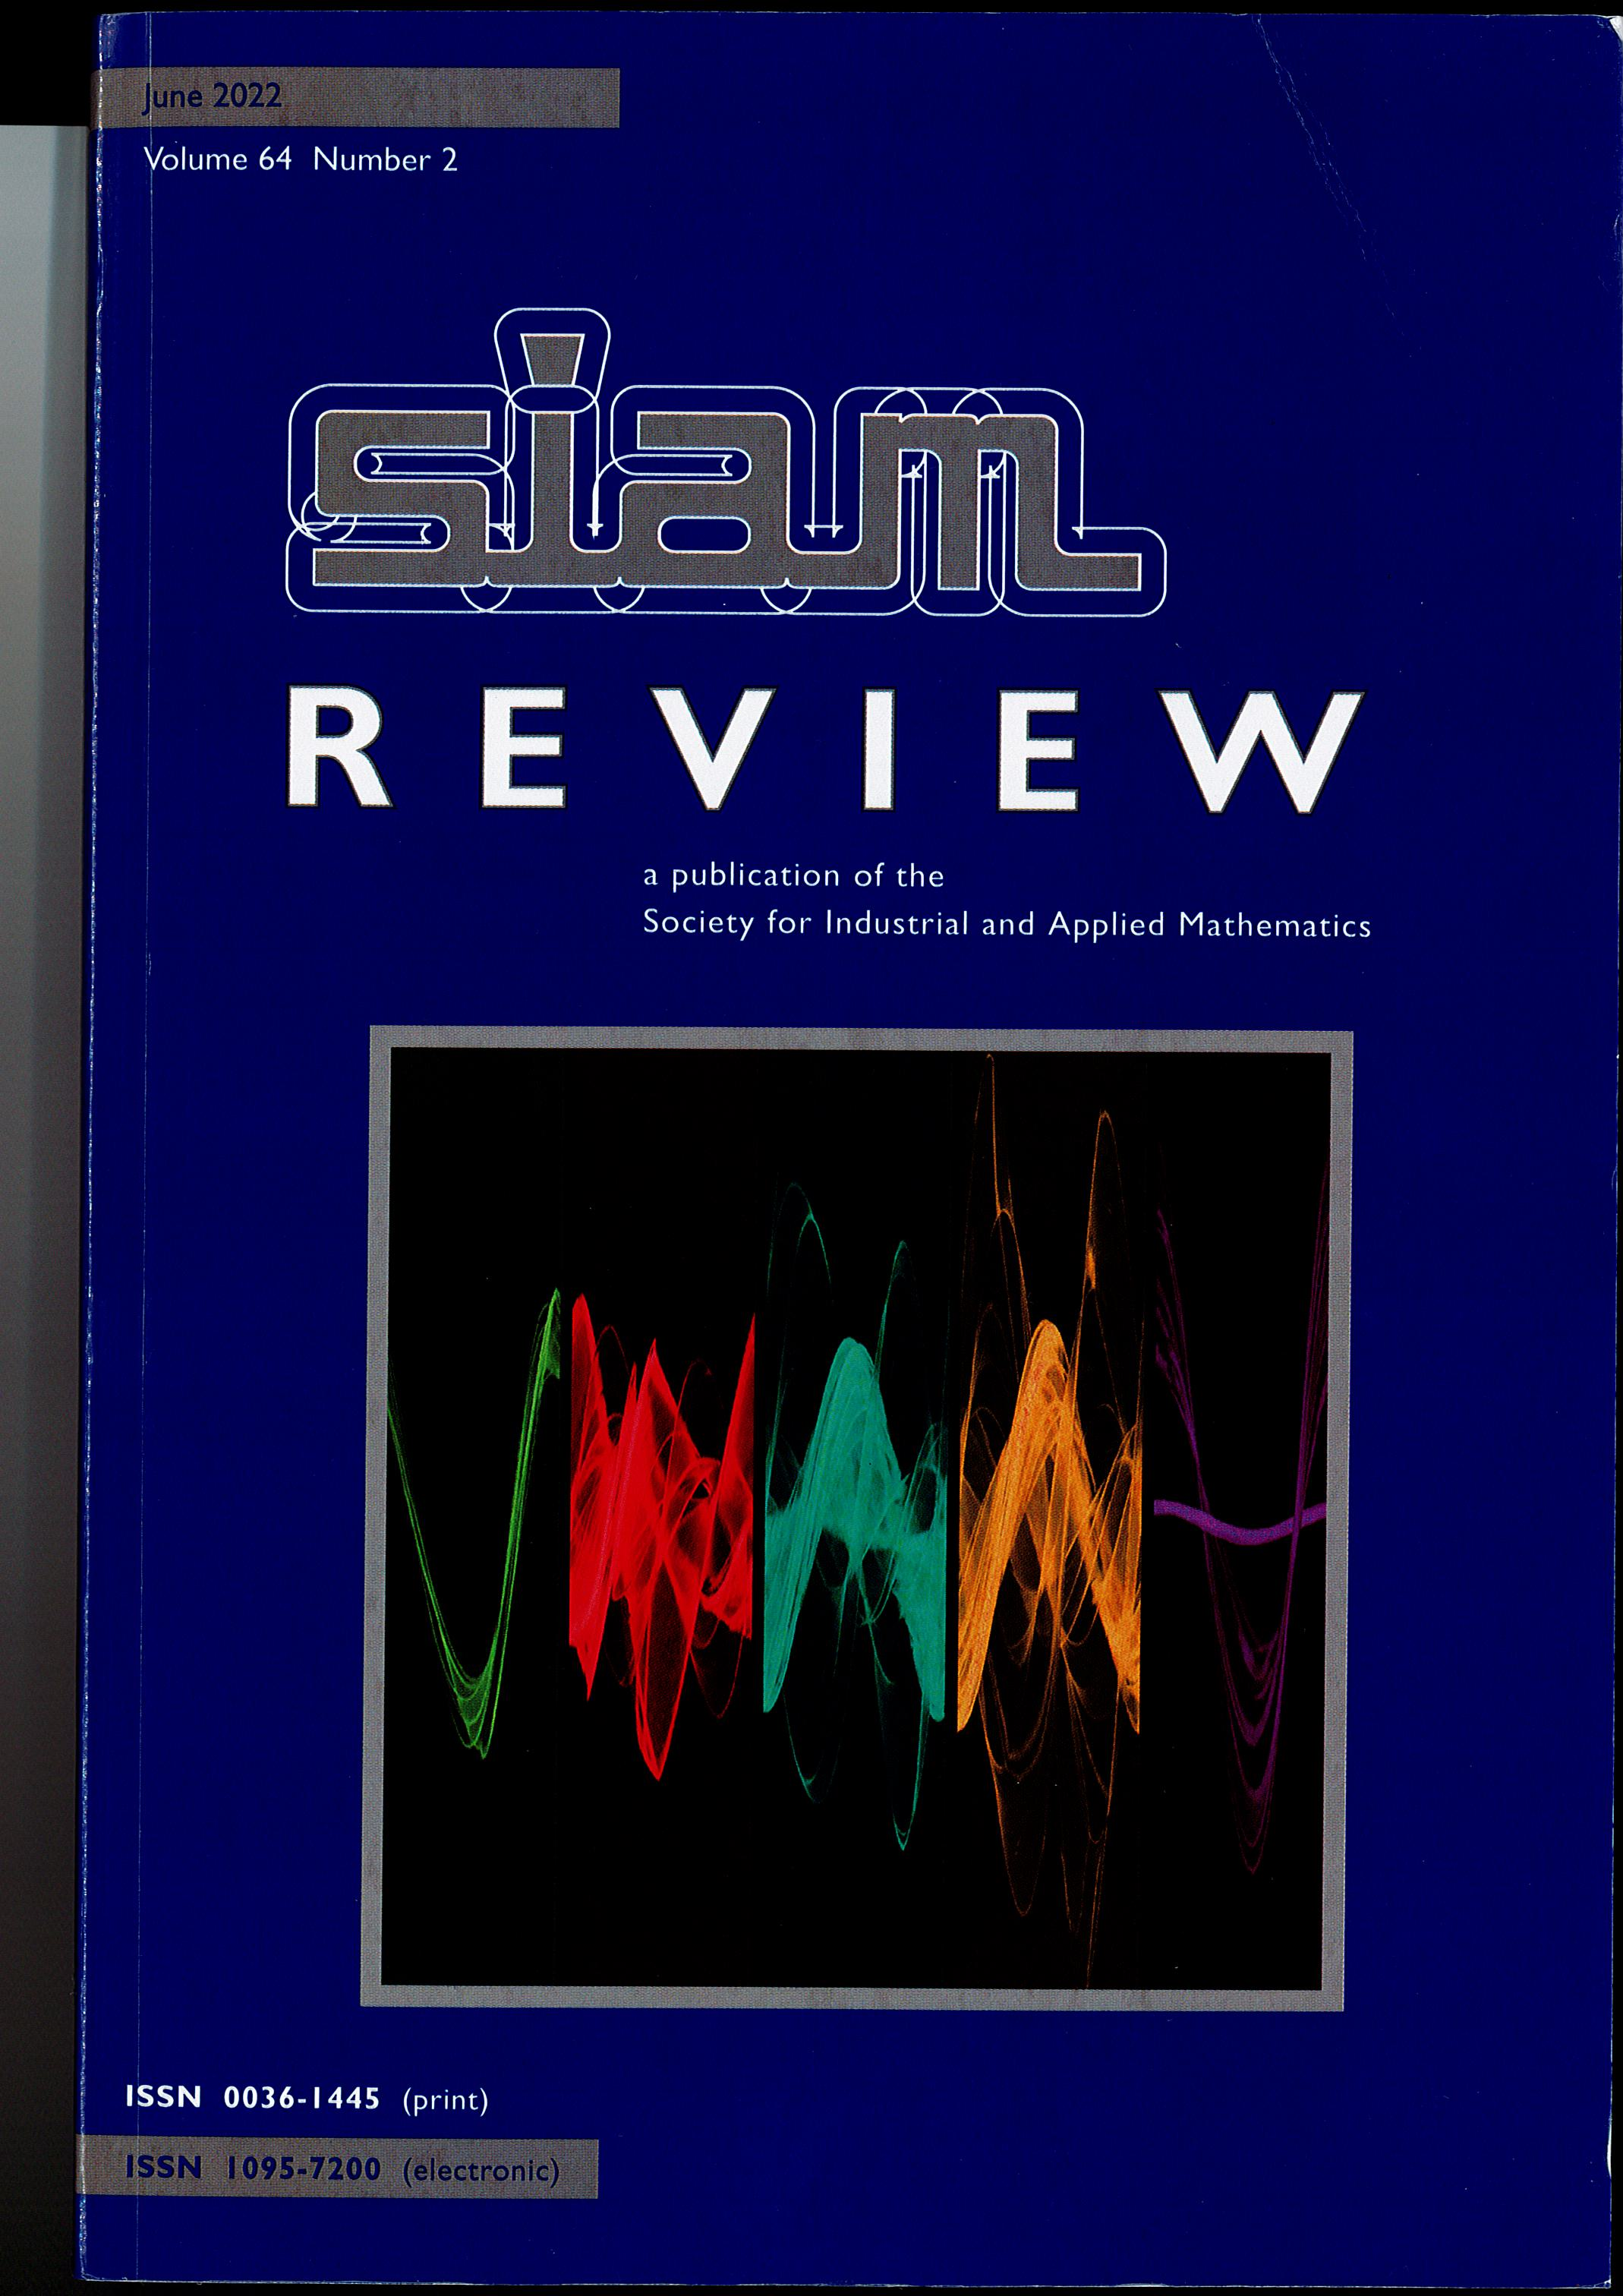
\includegraphics[scale=0.35]{../Figures/siam_new.jpg}
			%	\end{subfigure}
	\end{figure}	
\end{frame}	



	%\begin{frame}{Fourier Transform}
	%	\begin{figure}[h]
		%	\centering
		%	%	\begin{subfigure}{0.4\textwidth}
			%		%		\centering
			%		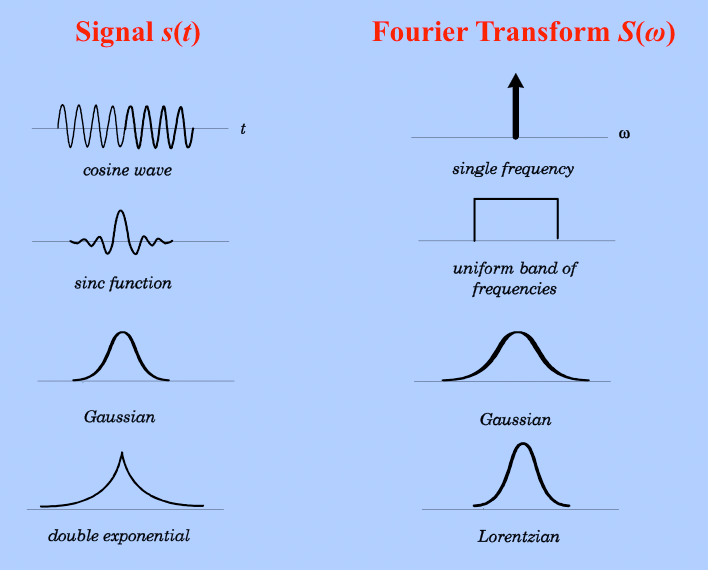
\includegraphics[scale=0.65]{../Figures/fig_fourier_transform.}
			%		%	\end{subfigure}
		%\end{figure}
		%\end{frame}
		
		
		%\begin{frame}{References}
		%	Materials and some of the pictures are from \citep{calin}.
		%	\printbibliography 	
		
		%	I have used some of the graphs by hacking TiKz code from StakExchange, Inkscape for more aesthetic plots and other old tricks of \TeX
		
		%\end{frame}
		
		
	\end{document}
